\section{Processing Guarantees}

	\noindent\textbf{Definition:} we have three modes of guarantees 
	\begin{itemize}
		\item at most once (weakest) : guaranteeing each message is processed at most once with a chance of getting lost
		\item at least once: guaranteeing processing each message at least once, with a chance of reprocessing some of the messages
		\item exactly once (strongest): guaranteeing each message being processed exactly one (no loss or reprocessing)
	\end{itemize}	 

	\noindent \textbf{Purpose:} This BB adds guarantees to the processing. Also, provides a mean to trade-off between performance and precise computing. As shown in \ref{fig:guarantees}, "at-most-once provides higher performance with lower latency and higher throughput, with more overhead being added as moving to "exactly-once". However, this comes at a cost of less precise processing with the possibility of loosing messages or processing the same message multiple times.
	
	\begin{figure}[h]
		\centering
		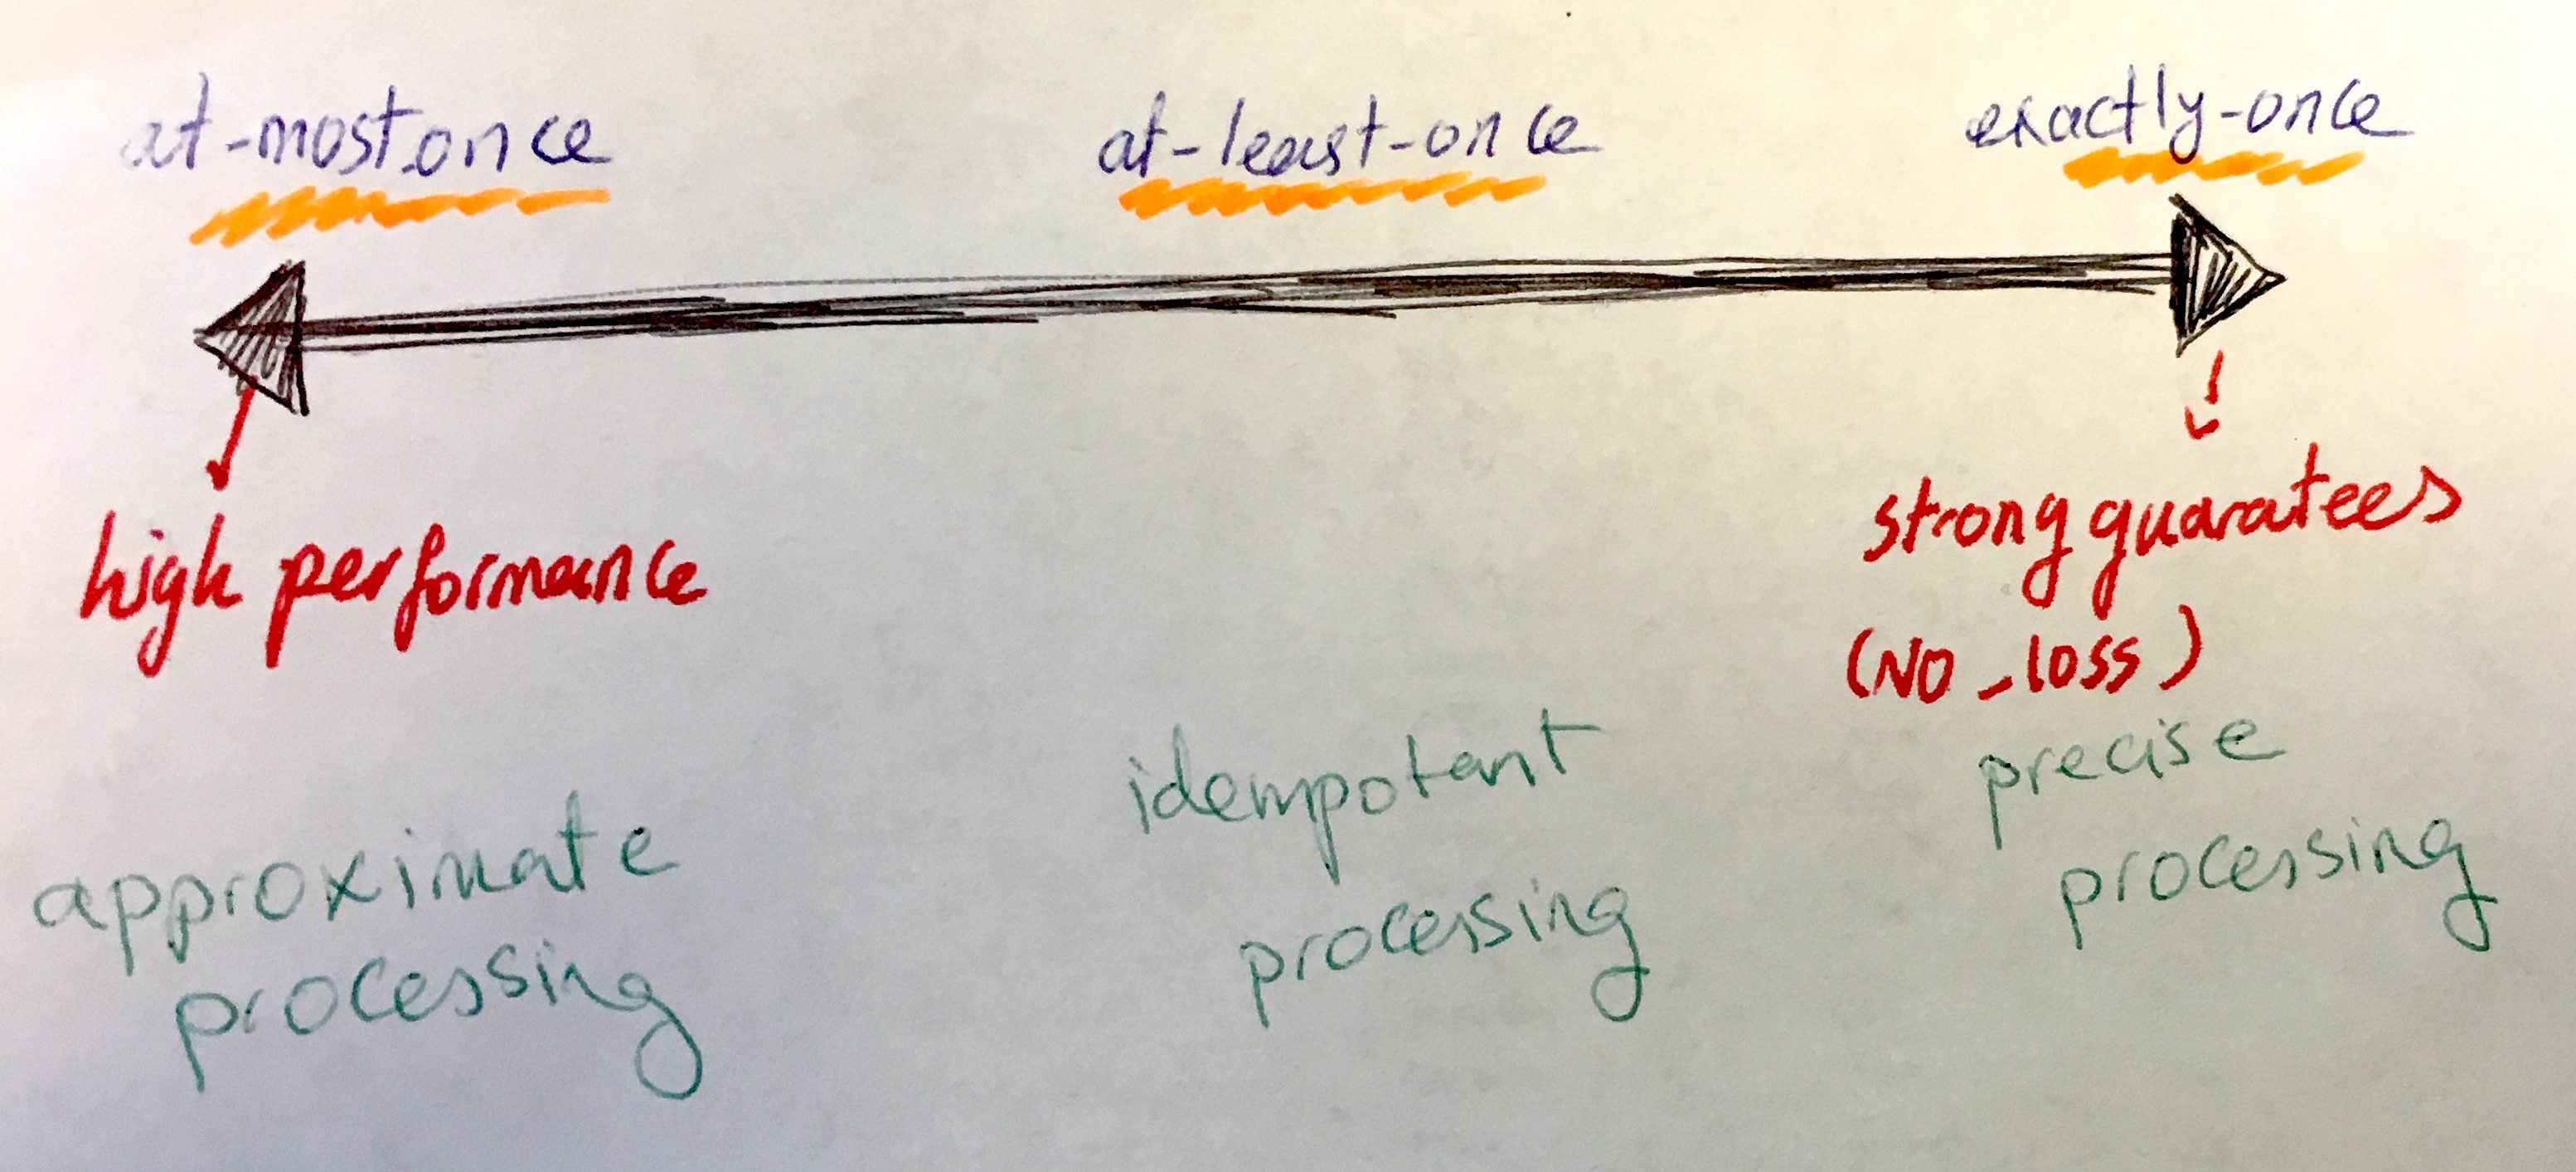
\includegraphics[width=0.45\linewidth]{guarantees.jpg}
		\caption{Spectrum of various guarantees and the trade-off among them. \Fix{redraw a nice figure.}}
		\label{fig:guarantees}
	\end{figure}
	
	
	\noindent \textbf{Usecase:} 
\\	\noindent \textbf{Techniques: }
\\	\noindent \textbf{Trade-off in techniques: } 
\\	\noindent \textbf{Future Direction:} 


Modes are:


\Fix{should the modes be  the spectrum or the mechanism to provide it?}

\Fix{What is the usecase of each mode? }
\Fix{is this section about these guarantees? or about techniques to provide each?}



